%!TEX root = ../farid_msc_thesis.tex

\chapter{Data and methodology}
\label{ch:methodology}

\section{Proposed Methodology for Ranking Business Models}
%
  We propose a pipeline (Fig. \ref{fig:pipeline}) for ranking business models, which is based on a Fuzzy Rule Inference System whose rules were created using previous data from the company (applications with an assigned score). \\
 The inputs for system created were the text applications itself, those who had to be parsed in order to extract the answers of questions. Those answers were preprocessed, and the words were projected into a vectorial space of 500 dimensions (this vectorial space were created to represent an Spanish language model). \\
 Finally, a compositional operation were applied to applications, in order to measure the "proximity" between the \textit{compositional text} and some \textit{key concepts} regarding an \textit{Design innovation} approach. After that, the "degree" of similarity between the \textit{compositional text} and \textit{key concepts} were the inputs to the Fuzz Rule Inference System, whose output is the score used to rank business applications. 
 
\begin{figure}[h]
	\label{fig:pipeline}
	\includegraphics[width=\textwidth]{Pipeline_textos.png}
    \caption{Proposed pipeline for ranking business models.}
\end{figure}

\subsection{Text applications}
Text data were \textit{scraped} from the company website. For this task, the \textbf{GNU Wget} package and \textbf{Beautifulsoup} python library were used in order to get data from HTML files. \\
At the end of this part, and PSV file (\textit{"pipe-separated values"}) was generated, where the answers for each question,  the ID and the final score (given by judges) of applications were stored in different columns.

On the other hand, our "secondary" source of text data were Wikipedia. So, we download a database of articles in Spanish \cite{wiki:Download} in order to create a model of the Spanish language. 

For both sources of text data, a list of common stop-words \cite{ranks:stopwords}, symbols, accents, numbers and links were removed using the \textbf{GNU sed} and \textbf{GNU tr}  command-line text editors. At the end of this step, most of text data consisted in words with relevant semantic meaning. 

A second pre-processing step consisted in implement a spelling-corrector algorithm, in order to avoid "words without meaning" due to typos.

Some statistics about length aplications are show below:

\texttt{.\\
count    8815.000000\\
mean     2152.153488\\
std       921.940859\\
min       213.000000\\
25\%      1491.000000\\
50\%      1970.000000\\
75\%      2601.000000\\
max      7340.000000\\
Name: length, dtype: float64\\}

In the next histogram (Fig. \ref{fig:allHistogram}), it is showed the histogram of length of applications, counting the number of words in each one. All answers from data applications were merged into one field, and the number of word of that field was assigned as a new ``length'' feature in the dataset. 

\begin{figure}[h]
	\label{fig:allHistogram}
	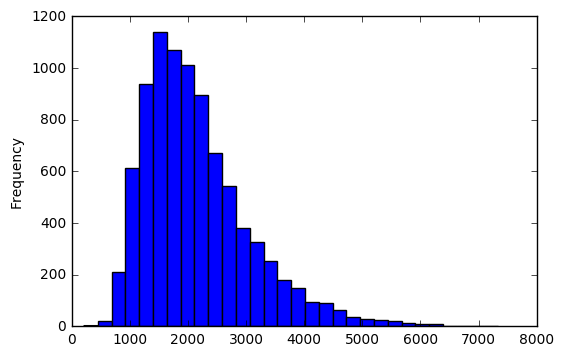
\includegraphics[width=\textwidth]{lengthApplications.png}
    \caption{Histogra of length of all applications.}
\end{figure}

Two more histograms (Fig. \ref{fig:clasesHistogram}) were created, in order to visualiza the lenght of applications according to the category they were assigned. The label ``-1'' was for those applications with overall scores less than 0 (assigned by \textit{expert judges}), and label ``+1''  with overall scores more than 0. 

\begin{figure}[h]
	\label{fig:clasesHistogram}
	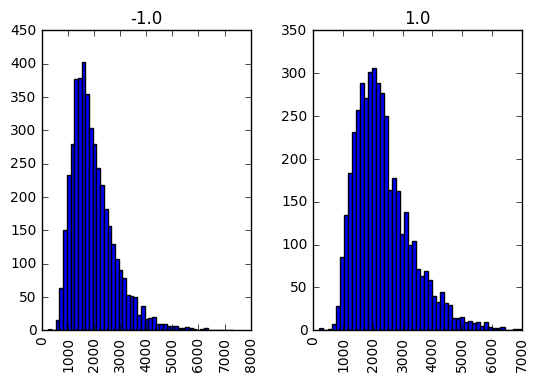
\includegraphics[width=\textwidth]{histogramClases.png}
    \caption{Histogram of length of applications, where Clase=-1 if they have a bad score, 1 otherwise.}
\end{figure}

\subsubsection{Spelling correction algorithm}
The spelling correction algorithm implemented in this work was developed by Peter Norving \cite{norvig2007write}. \\
\textbf{How many words were corrected?}
spellCorrectiongNorving

\subsubsection{Correlations between words and scores}
Bimodal distribution across scores, length of aplications is skewed to right.


\begin{figure}[h]
	\label{fig:correlaciones_tabla}
	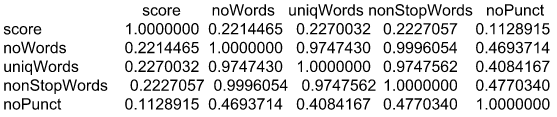
\includegraphics[width=\textwidth]{correlations_number_posible.png}
    \caption{There is not correlation between number of words, number of words without stop words or punctuations and score, in applications.}
\end{figure}

\begin{figure}[h]
	\label{fig:correlaciones}
	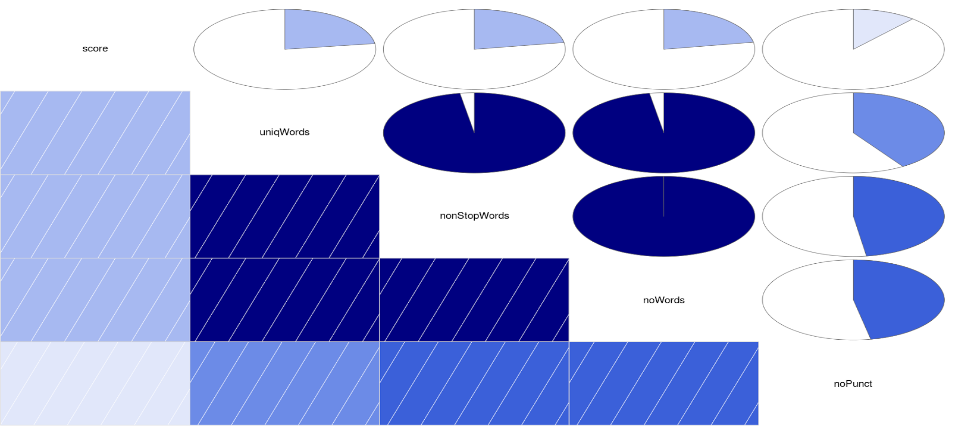
\includegraphics[width=\textwidth]{correlations_image_posible.png}
    \caption{There is not correlation between number of words, number of words without stop words or punctuations and score, in applications.}
\end{figure}

\subsection{Semantic Representation of Spanish Language}
	We generated a kind of Spanish "dictionary", preserving semantic properties of language, were each word is mapped into a vectorial space of 500 dimensions, using the Word Embedding algorithm implemented in \textit{Gensim} \cite{rehurek_lrec} python package.  This algorithm took as input the articles downloaded from Wikipedia, and the output was a file were each word was represented with a vector of 500 features. \\
	Singular Value Decomposition (SVD) was applied to a set of "key words", those with semantic meaning were related to \textit{Design Innovation} concepts, in order to visualize a proper relationship between our Spanish model.\textbf{insertar figura de SVD}.

\subsection{Accumulative Semantic Value by Topic}
Cosine distance

\subsection{Fuzzy Inference System}

\subsection{Discovering Rules for Ranking Application}
An Genetic approach

\subsection{Ranking Applications}


%
\subsection{Dataset Description}

